\documentclass[12pt,a4paper,titlepage]{article}
\usepackage[utf8]{inputenc}
\usepackage[T1]{fontenc}
\usepackage[top=3cm, bottom=3cm, left=2cm, right=2cm]{geometry}
\usepackage{textcomp}
\usepackage{amsmath}
\usepackage{amsfonts}
\usepackage{amssymb}
\usepackage{amsthm}
\usepackage{titlesec}
\usepackage{fancyhdr}
\usepackage{lastpage}
\usepackage{fix-cm}
\usepackage{graphicx}
\usepackage{hyperref}
\usepackage{xcolor}
\usepackage{mdwlist}
\usepackage{listings}
\usepackage{float}
\usepackage{wrapfig}
\usepackage{datetime}
\usepackage[perpage,para,bottom,marginal]{footmisc}
\usepackage{listings}
\usepackage{caption}
\usepackage{enumitem}
\usepackage{multicol}
\usepackage[cmtip,all]{xy}
\newdateformat{dmny}{\monthname[\THEMONTH] \THEYEAR}
\newdateformat{dyo}{\THEYEAR}
\setlength{\headheight}{30pt}
\pagestyle{fancy}

\author{Nicolas Hafner}
\lhead{Nicolas Hafner}
\title{Analysis II}
\chead{Analysis II}
\rhead{Zürich, \dmny\today}
\cfoot{\thepage\ / \pageref{LastPage}}
\lfoot{\copyright \dyo\today TymoonNET/NexT}
\date{\d_mny\today}

\newcommand{\longsquiggly}{\xymatrix{{}\ar@{~>}[r]&{}}}

\begin{document}	
\begin{center}{\bfseries\Huge Analysis II - 2014.02.20}\end{center}
\textit{Erinnerung}: $\frac{dy}{dx}=y^2$ Wo $y\neq0$ ist $y(x)$ lokal invertierbar \\
$\longsquiggly \frac{dx}{dy}=\frac{1}{y^2} \longsquiggly x=\int\frac{dy}{x^2}+c=c-\frac{1}{y}$ \\
\\
\textit{Beispiel}: $\frac{dy}{dx}=3\sqrt[3]{y^2}$ Wo $y\neq0$ ist, ist $y(x)$ lokal invertierbar $\longsquiggly \frac{dx}{dy}=\frac{1}{3y^{2/3}}=\frac{1}{3}y^{-2/3} $\\
$\longsquiggly x=\int\frac{1}{3}y^{-2/3}dy=y^{1/3}+c \longsquiggly (x-c)^3=y$ wo $y\neq0$ \\
\textit{Probe}: $\frac{d}{dx}((x-c)^3) = 3(x-c)^2 = 3((x-c)^3)^{2/3}=3(y)^{2/3} \longsquiggly$ Für jedes $c\in\mathbb{R}$ ist $\mathbb{R}\to\mathbb{R},\; x\mapsto(x-c)^3$ eine Lösung. Durch Einsetzen von $0$ erscheint eine weitere Lösung: $y\equiv 0$ identisch:\\
\begin{figure}[H]\centering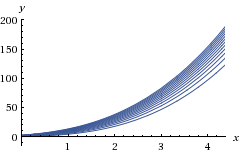
\includegraphics{WolframAlpha--dy_dx_3y__2_3___Sample_solution_family__2014_02_20_0332.png}\end{figure}
Die max. Lösungen sind dann genau die Funktionen $x\mapsto\left\{\begin{array}{l l}
    (x-c_2)^3 & \quad \text{für}\; x\geq x_2 \\
    0 & \quad \text{für}\; c_1<x<c_2 \\
    (x-c_1)^3 & \quad \text{für}\; x\leq c_1 \\
  \end{array}\right\}$ für $-\infty\leq c_1\leq c_2\leq\infty$.

\section*{Lösung durch Potenzreihenansatz}
\textit{Besipeil}: Besselsche DGL mit $n\in\mathbb{Z}^{\geq0}$:
$$f''(x)+\frac{1}{x}f'(x)+(1-\frac{n^2}{x^2})f(x)=0$$
Gesucht sind alle Lösungen $f(x)=\sum_k^\infty a_kx^k$ mit $a_k\in\mathbb{R}$ auf $]0,\varepsilon[,\;\varepsilon>0$. Wir benutzen dies nun als Ansatz und bestimmen die $a_k$.
$$\sum\limits_{k=0}^\infty k(k-1)x^{k-2}+\frac{1}{x}\sum\limits_{k=0}^\infty a_kkx^{k-1}+(1-\frac{n^2}{x^2}\sum\limits_{k\geq0} a_kx^k=0$$
$$\sum\limits_{l=0}^\infty a_{l+2}(l+2)(l+1)x^l+\frac{1}{x}\sum\limits_{l=-1}^\infty a_{l+2}(l+2)x^l+\sum\limits_{l\geq0}a_lx^l-\sum\limits_{l=-2}^\infty a_{l+2}n^2x^{l+2}=0$$
$$\sum\limits_{l=0}^\infty(a_{l+2}(l+2)(l+1)+a_{l+2}(l+2)+a_l-a_{l+2}n^2)x^l+(a_11-a_1n^2)x^{-1}+(-a_0n^2)x^{-2}=0$$
Jede dieser Klammerteile kann nun nach $0$ aufgelöst werden.
$$\iff n^2a_0=0 \quad\quad (n^2-1)a_1=0 \quad\quad \forall l\geq0: a_l+a_{l+2}((l+2)^2-n^2)=0$$
$$\iff \forall k\geq2: a_{k-2}=(n^2-k^2)a_k \Rightarrow n\geq0 \longsquiggly \forall k\neq n: a_k=\frac{a_{k-2}}{n^2-k^2}$$
$\Rightarrow \forall k\geq0 \;\text{mit}\; k\not\equiv n\mod2, \longsquiggly a_k=0$\\
$\Rightarrow \forall k\geq0 \;\text{mit}\; k\equiv n\mod2: \text{Für}\; k<n \;\text{folgt ebenso}\; a_k=0$\\
$k=n,\; a_{n-2}=0 \quad\quad k=n+2l,\; l\in\mathbb{Z}^{\geq0}$\\
$\Rightarrow a_{n+2l}=\frac{a_{n+2l-2}}{(n^2-(n+2l)^2)} = \frac{a_{n+2l-2}}{(2n+2l)(-2l)} = \frac{a_n}{(2n+2l)(2n+2l-2)..(2n+2) \cdot (-2l)(-2l+2)..(-2)} = \frac{a_n\cdot n!}{(n+l)!\cdot 2^l\cdot (-1)^l\cdot 2^l\cdot l!}$\\
$$\Rightarrow f(x)=\sum\limits_{k=0}^\infty a_kx^k=\sum\limits_{l=0}^\infty\frac{a_nn!}{(-1)^l\cdot 4^l\cdot (n+l)!\cdot l!}x^{n+2l}$$
\textit{Definition}: $n$-te Besselfunktion erster Art $Y_n(x):=\sum\limits_{l=0}^\infty\frac{x^{n+2l}}{(-4)^l(n+l)!l!}$ \\
Der Konvergenzradius ist $\infty$.

\section*{Seperierbare DGLen}
$\frac{dy}{dx}=y'=g(x)h(y) \iff \frac{dy}{h(y)}=g(x)dx \Rightarrow \int\frac{dy}{h(y)}=\int g(x)dx \Rightarrow H(y)=G(x)+c$\\
$\longsquiggly y=H^{-1}(G(x)+c)$\\
\\
\textit{Beispiel}: $\frac{dy}{dx}=1+y^2 \Rightarrow \int\frac{dy}{1+y^2}=\int dx \Rightarrow \arctan y = x+c \Rightarrow y=\tan(x+c)$ \\
\textit{Probe}: $\frac{d}{dx}(\tan(x+c))=\frac{1}{\cos^2(x+c)}=\frac{\sin^2+\cos^2}{\cos^2}=1+\tan^2(x+c)$ \\
\\
\textit{Beispiel}: $\frac{dy}{dx}=\sqrt{\frac{1-y^2}{1-x^2}},\; x,y\in]-1,1[ \Rightarrow \int\frac{dy}{\sqrt{1-y^2}}=\int\frac{dx}{\sqrt{1-x^2}} \Rightarrow \arcsin y=\arcsin x+c$\\
$\Rightarrow y=\sin(\arcsin x+c)=\sin(\arcsin x)\cos c+\cos(\arcsin x)\sin c = x\cos c+\sqrt{1-x}^2\sin c$ \\
$\Rightarrow y=ax+b\sqrt{1-x^2}$ für $a,b\in\mathbb{R}$ mit $a^2+b^2=1$.\\

\end{document}